% Indicate the main file. Must go at the beginning of the file.
% !TEX root = ../main.tex

%%%%%%%%%%%%%%%%%%%%%%%%%%%%%%%%%%%%%%%%%%%%%%%%%%%%%%%%%%%%%%%%%%%%%%%%%%%%%%%%
% 04_discussion
%%%%%%%%%%%%%%%%%%%%%%%%%%%%%%%%%%%%%%%%%%%%%%%%%%%%%%%%%%%%%%%%%%%%%%%%%%%%%%%%


\section{Discussion}
\label{discussion}

\subsection{Detection}


The detection process significantly influenced the dataset composition, particularly for the category \textit{mustela\_erminea}.
This category experienced higher data loss likely due to the species relative size --- it is much larger then the other species captured by this MammaliaBox camera traps.
This larger size may have resulted in more frequent bad shots dew to the closeness to the camera or the speed they pass trough the box --- a lot of images where showing only the tip of the animal's tail disappearing out of the box.
An other interesting observation was the fact that the white fur individuals were more often not detected than the brown fur individuals.
An explanation has yet to be found fot the fact that this was only the case for the sequence level, where the \textit{mustela\_erminea} category was disproportionally effected.
On the image level the \textit{soricidae} category was the most affected one with \(23\%\) of the images lost but only \(1\%\) of the sequences.

Visual inspection revealed a mixture of exemplary BBox detections alongside notable inaccuracies, such as missed detections in images with obstructions or partial visibility of animals.
Looking trough missclassified images with high confidence values, revealed some interessting insights.
One was that quite a few false positive detections were made and lead to surprisingly high confidence value classifications.
Some of these images were empty or contained no animal at all, as shown in \autoref{fig:false_positive_dt} showing some plant parts missdetected, some possibly animals in very dark areas of the image or some very small not really visible things.
An other interessting find was that quite some of the images contained a snail in the highest confidence BBox --- refer to \autoref{fig:false_class_snails} for a hand-picked selection of these examples.
These misclassifications, highlight the need for enhanced object discrimination capabilities or the introduction of an additional class for non-target species.

\begin{figure}[]
\centering
\includegraphics[width=\textwidth]{figures/false_positive_dt.pdf}
\caption{Hand-picked selection of images with a high confidence value but no animal in the image.}
\label{fig:false_positive_dt}
\end{figure}

\begin{figure}[]
\centering
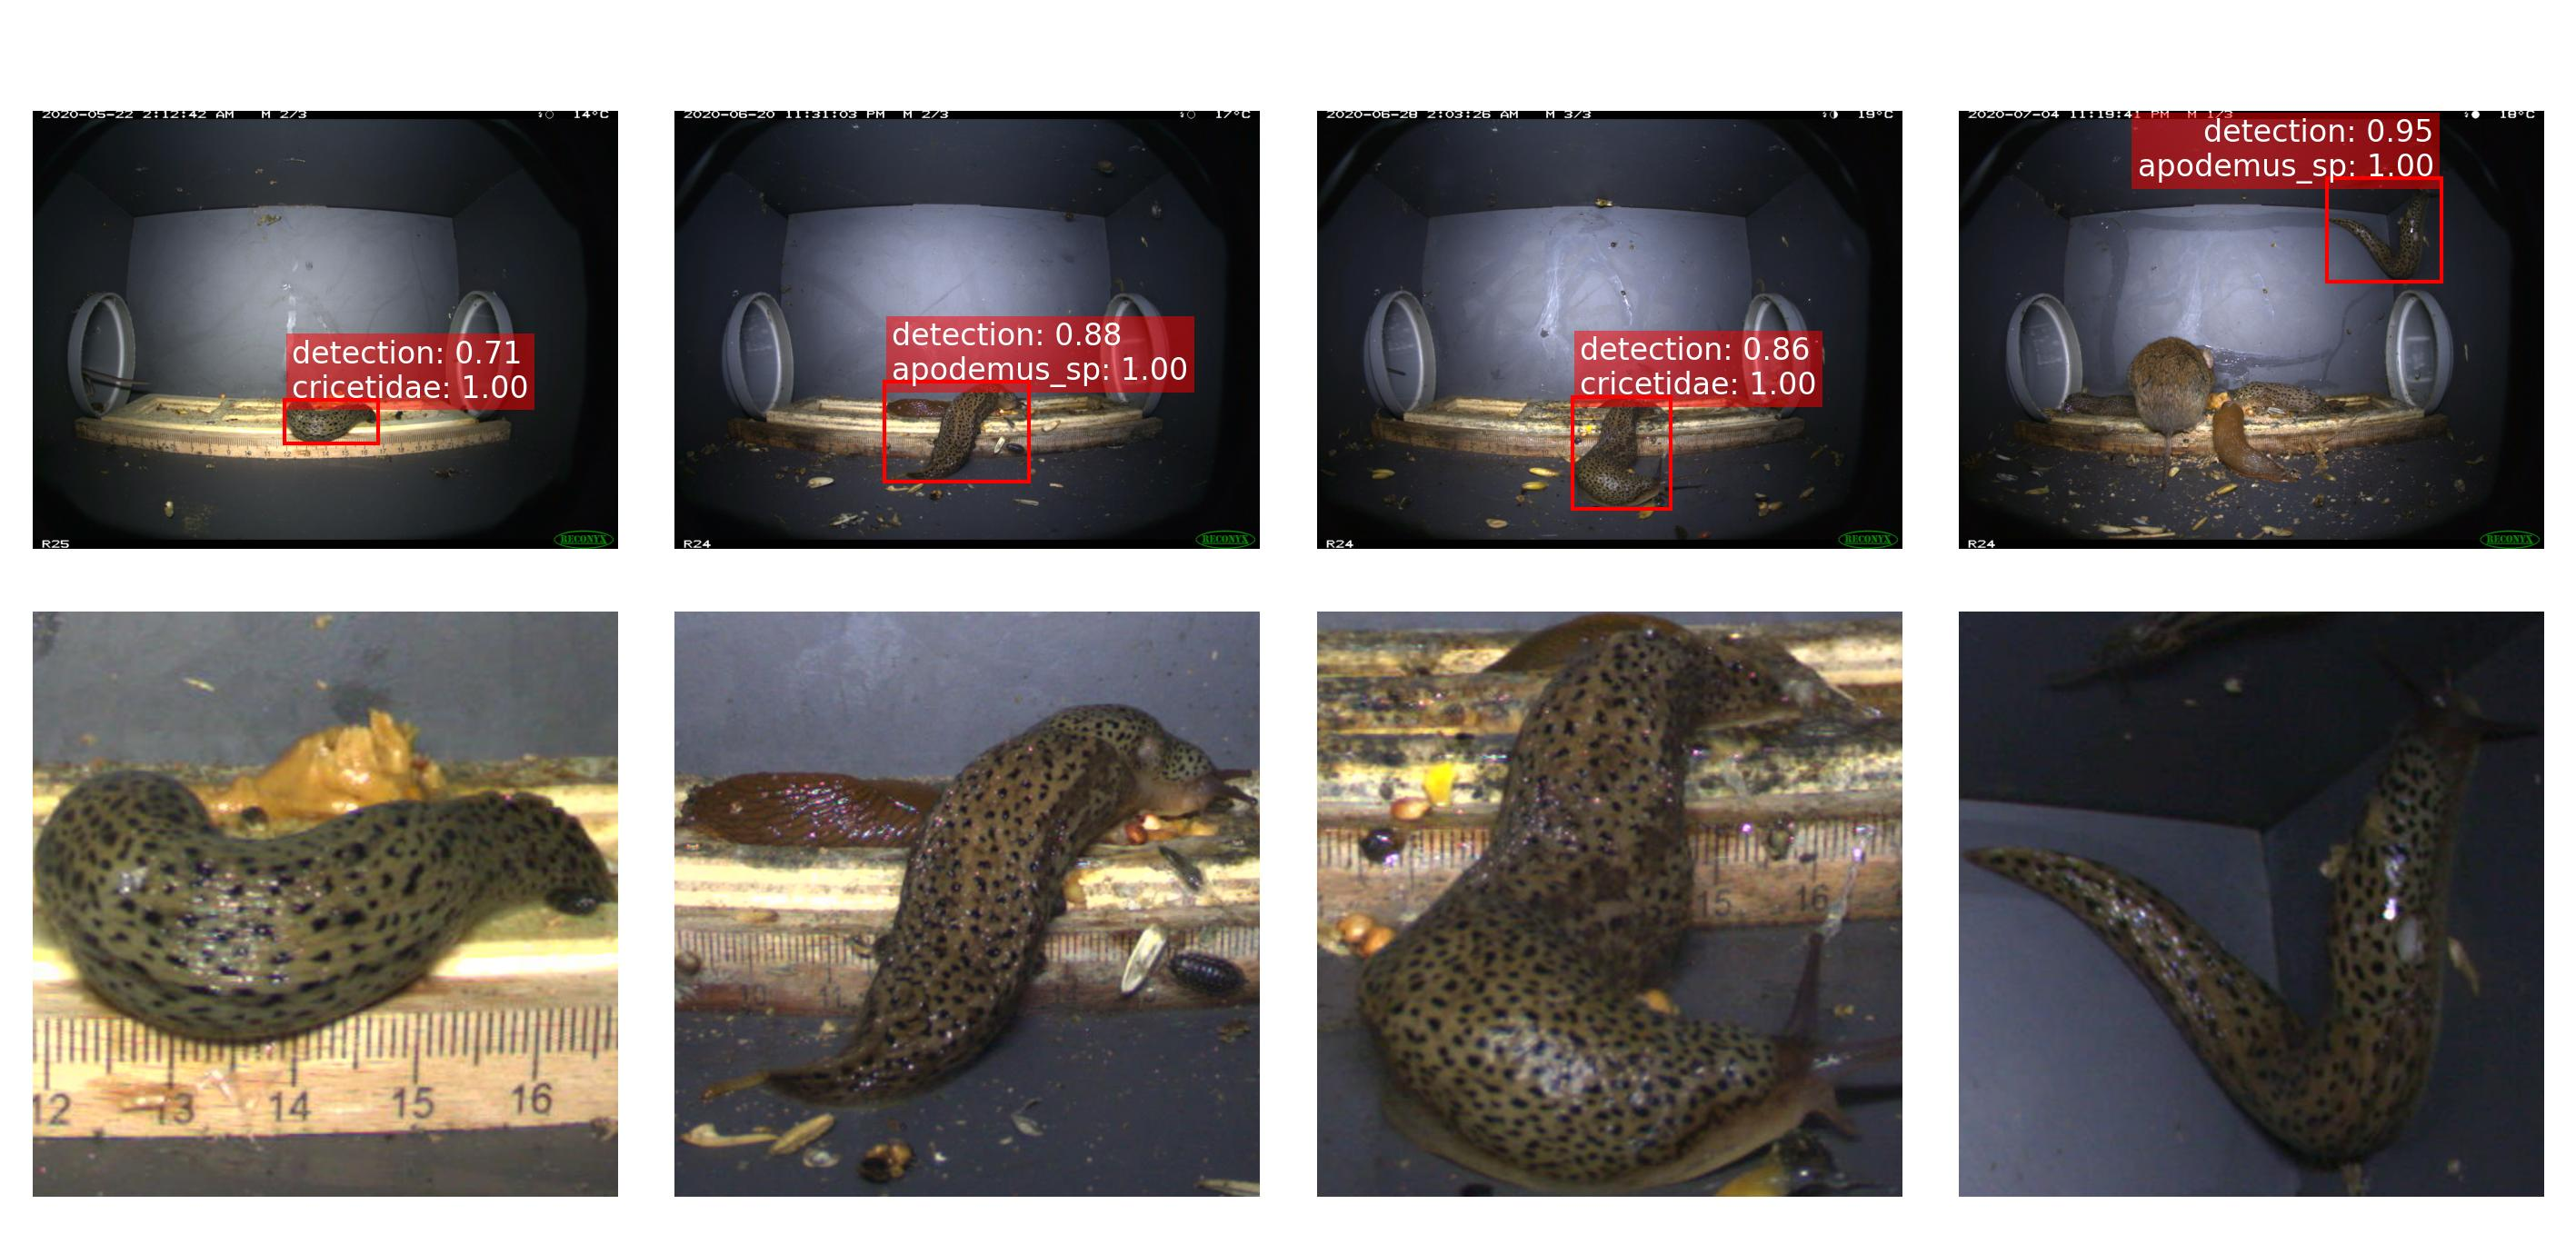
\includegraphics[width=\textwidth]{figures/false_class_snails.pdf}
\caption{Hand-picked selection of images predicted incorrectly with a high confidence value displaying a snail in the highest confidence BBox.}
\label{fig:false_class_snails}
\end{figure}

\subsection{Model Performance}
Overall, all tested models achieved high performance in image classification tasks, demonstrating their suitability for automating small mammal identification.
Pretrained models slightly outperformed those trained from scratch, underscoring the value of transfer learning.
The slight better balanced accuracy of pretrained models is just one of the benefits of using pretrained models, as they also require less training time and computational resources and could potentially be trained with less training data.

Interestingly, the smaller the models the better they performed on the image level classification task highlighting the fact that bigger is not always better.
Smaller models, if complex enough for the task are always preferable since they require less computational resources and are faster to train.
Examining \autoref{fig:bal_acc_img} again one could speculate about a trend for smaller models to perform more consistently across folds when trained from scratch --- but for some reason this is not the case for the EfficientNet-B0 model.
The observation for this study suggests smaller, computationally efficient models are sufficient and therefor preferable for the classification tasks.

\subsection{Best Model}

The pretrained EfficientNet-B0 emerged as the best-performing model, achieving the highest balanced accuracy.
Remarkably, optimal performance was reached within the first few training epochs.
Since the training dataset was quite large, only contained four classes and was intensively vetted using the MegaDetector, the model was able to learn the task quite quickly.
The observed weak but statistically significant correlation between detection confidence and classification confidence suggests that improved detections may lead to slightly better predictions.
However, since this correlation is very weak, the exploration of other factors influencing classification confidence might be beneficial.
The fact that overall classification confidence values were generally high, even for incorrect classifications and trough all detection confidence values, as shown in \autoref{fig:pred_conf_hexbin}, is again an indication that an additional class for non-target species would be beneficial.

\begin{figure}[]
\centering
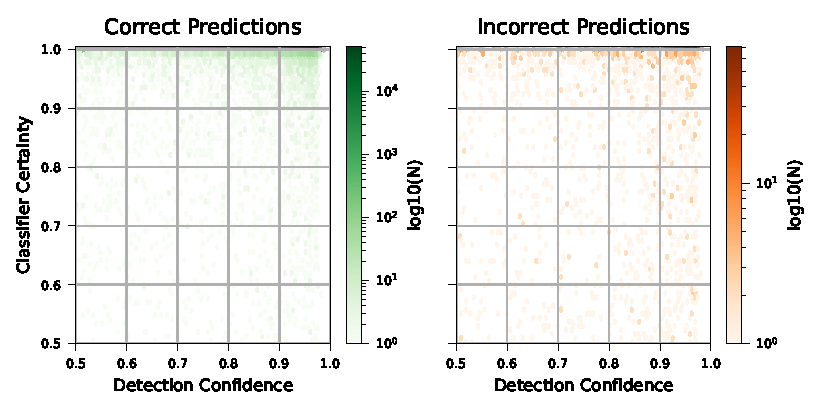
\includegraphics{figures/pred_conf_hexbin.pdf}
\caption{Hexbin plot of detection confidence vs. classifier certainty for correct and incorrect classifications. Color scale indicates log$_{10}$-binned counts.}
\label{fig:pred_conf_hexbin}
\end{figure}

\subsection{Limitations}

The primary limitation of the current methodology is the absence of an explicit non-target class, forcing models into potentially incorrect predictions, exemplified by the snail misclassification issue, shown in \autoref{fig:false_class_snails}.
Further, despite improvements, the MegaDetector still misses a significant number of potentially relevant detections.
This limitation is particularly pronounced for rare species, where insufficient data reduces detection reliability.
The loss of sequences for the \textit{mustela\_erminea} category, as shown in \autoref{tab:data_availability_after_md}, illustrates this issue.
Every sequence completely lost is a potentially missed sighting of a rare species, which could have provided valuable insights for conservation efforts.

Moreover, the current approach is heavily dependent on data availability.
Rare species inherently have fewer data points, constraining model training and potentially biasing predictions.

Lastly, although data augmentation techniques --- proven effective in improving model performance and generalization \autocite{shortenSurveyImageData2019} --- were initially considered, they were not employed.
Future work could revisit these techniques to potentially enhance robustness and accuracy.

Standardizing sequence lengths based on typical camera settings, such as 1, 3, 5, or 10 images per trigger, may further streamline future data processing and model training pipelines.
